\documentclass{beamer}
\usepackage{amsmath}
\usepackage{amssymb}
\usepackage{amsthm}                                        
\usepackage{textcomp}     
\usepackage{xcolor}
\usepackage{listings} 
\usetheme{Madrid}
\title{Quaternion Convolutional Neural Networks}
\author{Xuanyu Zhu\and Yi Xu \and  Hongteng Xu\and Changjian Chen}
\date{\today}
\begin{document}

\begin{frame}
    \titlepage
\end{frame}

% \begin{frame}
%     \frametitle{Table of Content}
%     \tableofcontents
% \end{frame}

\section{Introduction}
\begin{frame}
    \frametitle{Introduction}

    As a powerful feature representation method, convolutional neural networks (CNNs) have been widely applied in the field of computer vision. 
    \\~\\
    One key module of CNN model is the convolution layer, which extracts features from high-dimensional structural data efficiently by a set of convolution kernels. 
    \\~\\
    When dealing with multi-channel inputs (e.g., color images), the convolution kernels merges these channels by summing up the convolution results and output one single channel per kernel accordingly.
\end{frame}


\begin{frame}
    \frametitle{Introduction}
    \begin{figure}[H]
        \centering
        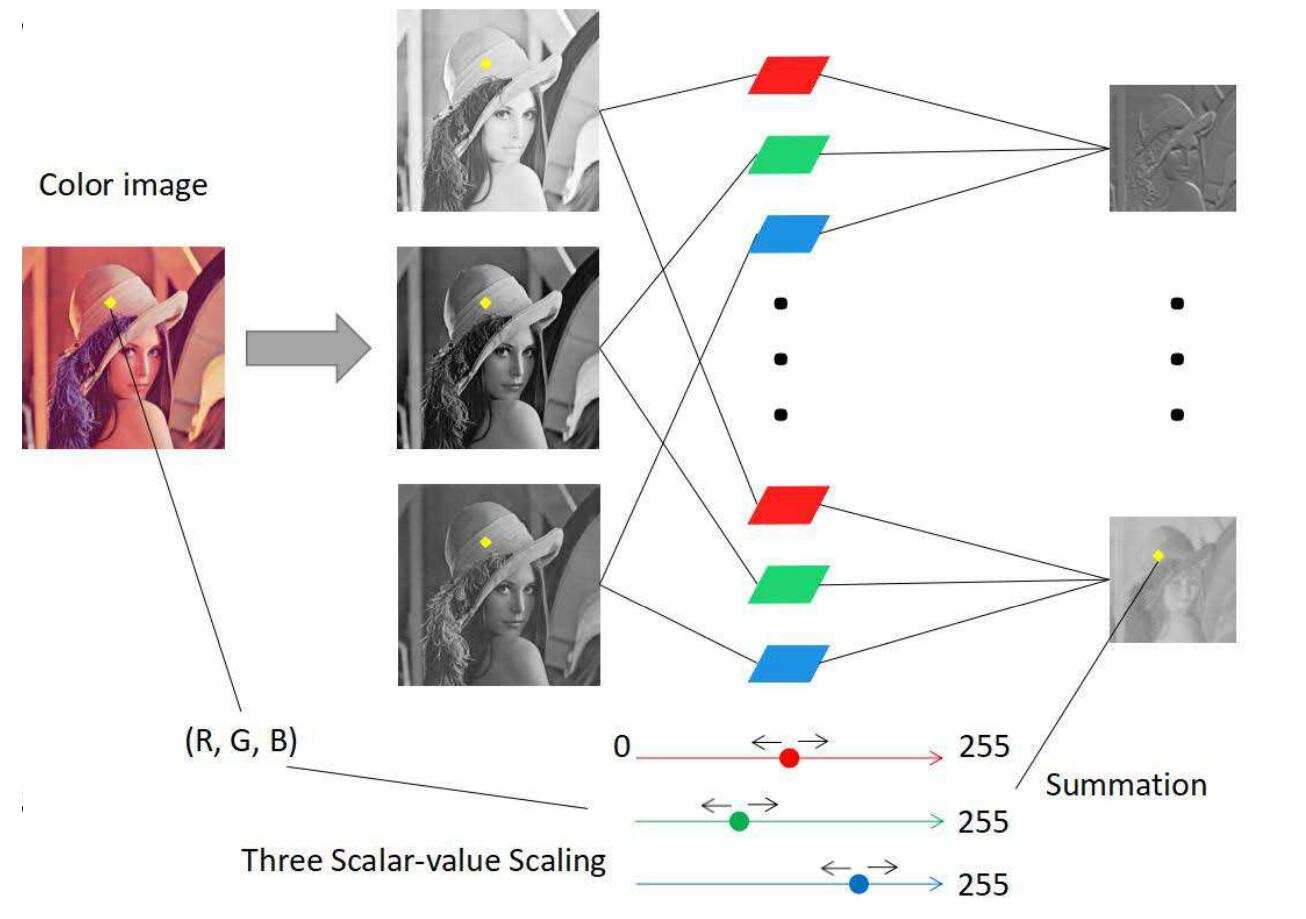
\includegraphics[width=.7\textwidth]{img/pic1.jpg}
        \caption{Real-valued CNN}
    \end{figure}
\end{frame}

\begin{frame}
    \frametitle{Introduction}

    We may lose important structural information of color and obtain non-optimal representation of color image.
    \\~\\
    Simply summing up the outputs gives too many degrees of freedom to the learning of convolution kernels.
    \\~\\
    We may have a high risk of over-fitting even if imposing heavy regularization terms.
\end{frame}

\begin{frame}
    \frametitle{Introduction}

    We propose a novel quaternion convolutional neural network (QCNN) model, which represents color image in the quaternion domain.
    \\~\\
    While the traditional real-valued convolution is only capable to enforce scaling transformation on the input, specifically, the quaternion convolution achieves the scaling and the rotation of input in the color space, which provides us with more structural representation of color information.
    \\~\\
    We establish fully-quaternion CNNs to represent color images in a more effective way and study the relationship between our QCNN model and existing real-valued CNNs and find a compatible way to combine them together in a same algorithmic framework.
\end{frame}

\begin{frame}
    \frametitle{Introduction}
    \begin{figure}[H]
        \centering
        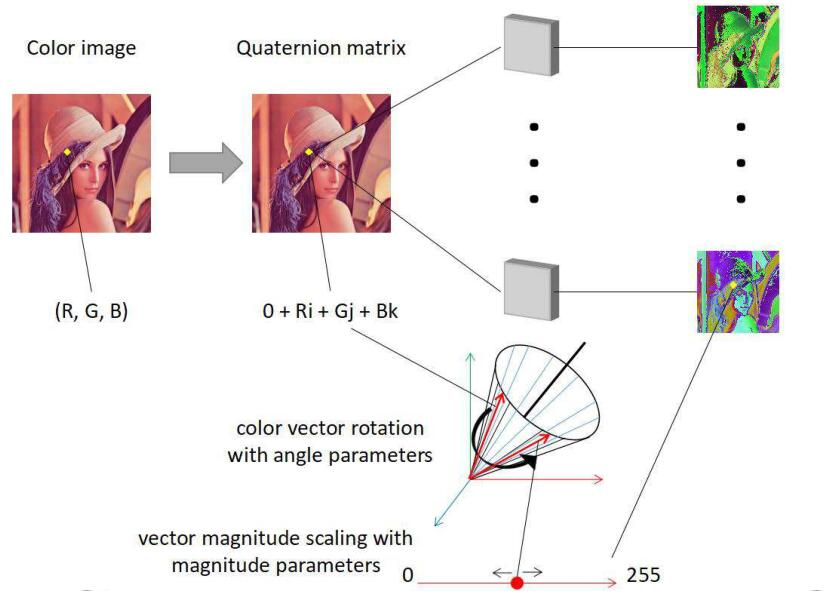
\includegraphics[width=.7\textwidth]{img/pic2.jpg}
        \caption{Quaternion CNN}
    \end{figure}
\end{frame}

\section{Related works}
\subsection{Quaternion-based color image processing}
\begin{frame}{Related works}{Quaternion-based color image processing}
    A quaternion $\hat{q}$ in the quaternion domain $\mathbb{H}$, \emph{i.e}, $q\in \mathbb{H}$, can be represented as $\hat{q}=q_0+q_1i+q_2j+q_3k$, where $q_i\in \mathbb{R}$ for $i=0,1,2,3$, and the imaginary units $i,j,k$ obey the quaternion rules that $i^2=j^2=k^2=ijk=-1$. Similar to real numbers, we can define a series of operations for quaternions:
\end{frame}

\begin{frame}{Related works}{Quaternion-based color image processing}
    \begin{itemize}
        \item Addition:
        \begin{equation*}
            \begin{split}
                \hat{p}+\hat{q}=&(p_0+q_0)+(p_1+q_1)i\\
                                +&(p_2+q_2)j+(p_3+q_3)k
            \end{split}
        \end{equation*}
        \item Scalar multiplication: $$\lambda \hat{q}=\lambda q_0+\lambda q_1i+\lambda q_2j+\lambda q_3k$$
        \item Element multiplication: 
        \begin{equation*}
            \begin{split}
                \hat{p}\hat{q}=&(p_0q_0-p_1q_1-p_2q_2-p_3q_3)\\
                            +&(p_0q_1+p_1q_0+p_2q_3-p_3q_2)i\\
                            +&(p_0q_2-p_1q_3-p_2q_0-p_3q_1)j\\
                            +&(p_0q_3+p_1q_2-p_2q_1-p_3q_0)k
            \end{split}
        \end{equation*}
    \end{itemize}
\end{frame}

\begin{frame}{Related works}{Quaternion-based color image processing}
    \begin{itemize}
        \item Conjugation: $$\hat{q}^*=q_0-q_1i-q_2j-q_3k$$
    \end{itemize}
    These quaternion operations can be used to represent rotations in a three-dimensional space. Suppose that we rotate a 3D vector $\textbf{q}=[q_1,q_2,q_3]^T$ to get new vector $\textbf{p}=[p_1,p_2,p_3]^T$, with an angle $\theta$ and along a rotation axis $\textbf{w}=[w_1,w_2,w_3]^T, w_1^2+w_2^2+w_3^2=1$. Such a rotation is equivalent to the following
    quaternion operation:
    \begin{equation}
        \hat{p}=\hat{w}\hat{q}\hat{w}^*
    \end{equation}
    where $\hat{q}= 0 + q_1i + q_2j + q_3k$, $\hat{p}= 0 + p_1i + p_2j + p_3k$ and 
    \begin{equation}
        \hat{w}=\cos\frac{\theta}{2}+\sin\frac{\theta}{2}(w_1i + w_2j + w_3k)
    \end{equation}
\end{frame}

\subsection{Real-valued CNNs and their extensions}
\begin{frame}{Related works}{Real-valued CNNs and their extensions}
Convolutional neural network is one of the most successful models in many vision tasks. CNNs have achieved encouraging results in many field like digit recognition, image classification, low-level vision.
\\~\\
Some efforts have been made to extend real-valued neural networks to other number fields. Complex-valued neural networks have been built and proved to have advantage on generalization ability and can be more easily optimized.
\\~\\
In \emph{Deep quaternion networks}, a deep quaternion
network is proposed. However, its convolution simply replaces the real multiplications with quaternion ones, and its quaternion kernel is not further parameterized. Our proposed quaternion convolution, however, is physically-meaningful
for color image processing tasks.

\end{frame}

\section{Proposed Quaternion CNNs}
\subsection{Quaternion convolution layers}
\begin{frame}{Proposed Quaternion CNNs}{Quaternion convolution layers}
Focusing on color image representation, our quaternion CNN treats a color image as a 2D pure quaternion matrix, denoted as $\hat{A}=[\hat{a}_{nn'}]\in \mathbb{H}^{N\times N}$ where $N$ represents the size of the image. In particular, the quaternion matrix $\hat{A}$ is 
\begin{equation}
    \hat{A}=\mathbf{0}+\textbf{R}i+\textbf{G}j+\textbf{B}k,
\end{equation}
where $\textbf{R},\textbf{G},\textbf{B}\in \mathbb{R}^{N\times N}$ represent red, green and blue channels, respectively.

\end{frame}

\begin{frame}{Proposed Quaternion CNNs}{Quaternion convolution layers}
Suppose that we have an $L\times L$ quaternion convolution kernel $\hat{W}=[\hat{w}_{ll'}]\in \mathbb{H}^{L\times L}$. We aim to design an effective and physically-meaningful quaternion convolution operation, denoted as $\circledast$ between the input $\hat{A}$ and kernel $\hat{W}$.
\\~\\
Specifically, this operation should
\begin{enumerate}
    \item apply rotations and scalings to color vectors in order to find the best representation in the whole color space; 
    \item play the same role as real-valued convolution when processing grayscale images.
\end{enumerate}
\end{frame}

\begin{frame}{Proposed Quaternion CNNs}{Quaternion convolution layers}
To achieve this aim, we take advantage of the rotational nature of quaternion shown in (1,2) and propose a quaternion convolution in a particular form. Specifically, we set the element of the quaternion convolution kernel as
\begin{equation}
    \hat{w}_{ll'}=s_{ll'}(\cos\frac{\theta_{ll'}}{2}+\sin\frac{\theta_{ll'}}{2}\mu)
\end{equation}
where $\theta_{ll'}\in [-\pi,\pi]$ and $s_{ll'}\in \mathbb{R}$. $\mu$ is the gray axis with unit length \emph{i.e}, $\frac{\sqrt{3}}{3}(i+j+k)$.
\end{frame}

\begin{frame}{Proposed Quaternion CNNs}{Quaternion convolution layers}
    The quaternion convolution is defined as
    \begin{equation}
        \hat{A}\circledast \hat{W} =\hat{F}=[\hat{f}_{kk'}]\in \mathbb{H}^{(N-L+1)\times (N-L+1)}
    \end{equation}
    where 
    \begin{equation}
        \label{e6}
        \hat{f}_{kk'}=\sum_{l=1}^L\sum_{l'=1}^L \frac{1}{s_{ll'}}\hat{w}_{ll'}\hat{a}_{(k+l)(k'+l')}\hat{w}^*_{ll'}
    \end{equation}
\end{frame}

\begin{frame}{Proposed Quaternion CNNs}{Quaternion convolution layers}
The advantage of such a definition is interpretable. The convolution in traditional CNNs operates triple scaling transforms to each pixel independently to walk through three color axes and it needs to find the best representation in the whole color space accordingly. 
\\~\\
For our QCNNs, one pixel is a quaternion or a 3D vector in color space, but the proposed convolution find its best representation in a small part of the color space because we restrict the convolution to apply only a rotate and a scaling transform.
\\~\\
Such a convolution actually impose implicit regularizers on the model, such that we can suppress the risk of over-fitting brought by too many degrees of freedom to the learning of kernels. 
\end{frame}

\begin{frame}{Proposed Quaternion CNNs}{Quaternion convolution layers}
Although our convolution operation is designed for color image, it can be applied to grayscale image as well. For grayscale images, they can be seen as color images whose channels are the same. Because all the corresponding color vectors are parallel to the gray axis, the rotate transform equals to identical transformation, thus the quaternion convolution performs the same function as real-valued convolution. From this viewpoint, real-valued convolution is a special case of quaternion convolution for grayscale image.
\end{frame}

\begin{frame}{Proposed Quaternion CNNs}{Quaternion convolution layers}
According to the rule of quaternion computations, if we represent each $\hat{a}_{nn'}$, as a 3D vector $\textbf{a}_{nn'}=[a_1,a_2,a_3]^T$, then the operation in \eqref{e6} can be represented by a set of matrix multiplications:
\begin{equation}
    \label{e7}
    \textbf{f}_{kk'}=\sum_{l=1}^L\sum_{l'=1}^Ls_{ll'}
    \begin{pmatrix}
        f_1&f_2&f_3\\
        f_3&f_1&f_2\\
        f_2&f_3&f_1\\
    \end{pmatrix}
    \textbf{a}_{(k+l)(k+l')}
\end{equation}
where $\textbf{f}_{kk'}$ is a vectorized representation of quaternion $\hat{f}_{kk'}$, and 
$$f_1=\frac{1}{3}+\frac{2}{3}\cos\theta_{ll'},f_2=\frac{1}{3}-\frac{2}{3}\cos(\theta_{ll'}-\frac{\pi}{3}),f_1=\frac{1}{3}-\frac{2}{3}\cos(\theta_{ll'}+\frac{\pi}{3})$$
\end{frame}

\begin{frame}{Proposed Quaternion CNNs}{Quaternion convolution layers}
    
\end{frame}





\end{document}
